\documentclass[a0paper,portrait]{baposter}

\usepackage{wrapfig}
\usepackage{lmodern}

\usepackage[utf8]{inputenc} %unicode support
\usepackage[T1]{fontenc}


\selectcolormodel{cmyk}

\graphicspath{{img/}} % Directory in which figures are stored

\newcommand{\compresslist}{%
\setlength{\itemsep}{0pt}%
\setlength{\parskip}{1pt}%
\setlength{\parsep}{0pt}%
}
\newcommand*{\pasp}{PASP}

\newenvironment{boenumerate}
  {\begin{enumerate}\renewcommand\labelenumi{\textbf\theenumi.}}
  {\end{enumerate}}



\begin{document}


\definecolor{darkgreen}{cmyk}{1,0.08,0,0.75}
\definecolor{lightgreen}{cmyk}{1,.12,0,0.27}

\begin{poster}
{
grid=false,
headerborder=open, % Adds a border around the header of content boxes
colspacing=1em, % Column spacing
bgColorOne=white, % Background color for the gradient on the left side of the poster
bgColorTwo=white, % Background color for the gradient on the right side of the poster
borderColor=darkgreen, % Border color
headerColorOne=lightgreen, % Background color for the header in the content boxes (left side)
headerColorTwo=lightgreen, % Background color for the header in the content boxes (right side)
headerFontColor=white, % Text color for the header text in the content boxes
boxColorOne=white, % Background color of the content boxes
textborder=rounded, %rectangle, % Format of the border around content boxes, can be: none, bars, coils, triangles, rectangle, rounded, roundedsmall, roundedright or faded
eyecatcher=false, % Set to false for ignoring the left logo in the title and move the title left
headerheight=0.11\textheight, % Height of the header
headershape=rounded, % Specify the rounded corner in the content box headers, can be: rectangle, small-rounded, roundedright, roundedleft or rounded
headershade=plain,
headerfont=\Large\textsf, % Large, bold and sans serif font in the headers of content boxes
%textfont={\setlength{\parindent}{1.5em}}, % Uncomment for paragraph indentation
linewidth=2pt % Width of the border lines around content boxes
}
{}
%
%----------------------------------------------------------------------------------------
%	TITLE AND AUTHOR NAME
%----------------------------------------------------------------------------------------
%
{
\textsf %Sans Serif
% \raggedleft
{Spectroscopic Data Reduction Pipeline for the Goodman High Throughput Spectrograph.
}
} % Poster title
% {\vspace{1em} Marta Stepniewska, Pawel Siedlecki\\ % Author names
% {\small \vspace{0.7em} Department of Bioinformatics, Institute of Biochemistry and Biophysics, PAS, Warsaw, Pawinskiego 5a}} % Author email addresses
{\sf\vspace{0.1em}\\
Sim\'on Torres-Robledo$^1$, C\'esar Brice\~no$^{1,2}$, and Bruno Quint$^1$
\vspace{0.1em}\\
\small{$^1$SOAR Telescope, La Serena, Regi\'on de Coquimbo, Chile.\\
$^2$Cerro Tololo Interamerican Observatory, Casilla 603, La Serena 1700000, Chile.
\vspace{0.2em}\\
storres@ctio.noao.edu}
}
{
\includegraphics[width=97px]{logo.eps}} % University/lab logo


\headerbox{1. Introduction}{name=introduction,column=0,row=0, span=3}{
The Goodman High Throughput Spectrograph (Goodman Spectrograph) \cite{2004SPIE.5492..331C} is a highly
versatile instrument in operation at the SOAR Telescope on Cerro Pach\'on, Chile.
It is capable of doing low to mid-resolution spectroscopy in a range from 3200 \AA{}
to 9000 \AA{}. The data reduction pipeline is conceived as an easy-to-run software,
that can process an entire night worth of data by execution of a simple command,
with the least amount of arguments, from a terminal window. It is written almost entirely in
Python, following several Python standard conventions.
We aim towards using exclusively standard Python packages, such as Astropy and
Astropy-affiliated packages, while at the same time allowing for fast and
efficient computing.
In its present form the pipeline produces fully reduced, wavelength-calibrated
spectra. Flux calibration will be an add-on option for a later release.
}


\headerbox{2. Scripts}{name=scripts,column=0,below=introduction,span=1}{

To describe a molecule, DeCAF substitutes its functional groups with pharmacophoric points (hence the "F" in the algorithm's name).
Points are organised into an undirected graph.
Lengths of the edges in the graph represents the number of bonds between pharmacophoric points.

% \begin{center}
%     \includegraphics[width=\linewidth]{phar}
% \end{center}
% %\vspace{-2pt}
}


\headerbox{3. Future Work}{name=future,column=0,below=scripts,span=1}{

The TODO list is large and the users and community input is very
important to help us decide were to focus our efforts. A list of the most
prominent changes are listed below. From the software point of view:


{\bf Structure:} The current static structure is confusing.
 There is a development version that includes a modified static structure more according
 to an Astropy Affiliated Package.\\
{\bf Tests:} Implement integrated test code. \\
{\bf Workflow:} Review the current workflow and propose an update.\\
{\bf User Manual:} Although we have a fully functional user manual we need feedback regarding how clear
 it is for non-regular users.

\vspace{.1in}
From the scientific point of view:

{\bf Extraction:} The current spectrum extraction is in fact a simple sum of counts
in a rectangular region. We will implement fractional pixel extraction as well as 
the Optimal Extraction algorithm \cite{1989PASP..101.1032M} \cite{1986PASP...98..609H}.

{\bf Operation:} We are planinig to develop a \emph{Live reduction pipeline} that 
can process data as it comes from the telescope that will allow observers to take quick decisions.

{\bf Telemetry:} Knowing how the pipeline and instrument behaves is very important to prevent failures. We
are developing a system to store the parameters of the wavelength solution polynomial
with the intention to validate new solution and eventually detect problems with the instrument.

}

\headerbox{4. Pipeline Concept}{name=concept,span=2,column=1,below=introduction}{ % To reduce this block to 1 column width, remove 'span=2'

We aimed to develop an easy to use software. A user should be able to run it with
the least amount of command line arguments yet it should allow a large enough 
flexibility to be usable in a wide range of configurations just as the Goodman
Spectrograph does. Also it should be built as a library in order to reuse the
code. 

\vspace{-5pt}
\begin{center}
    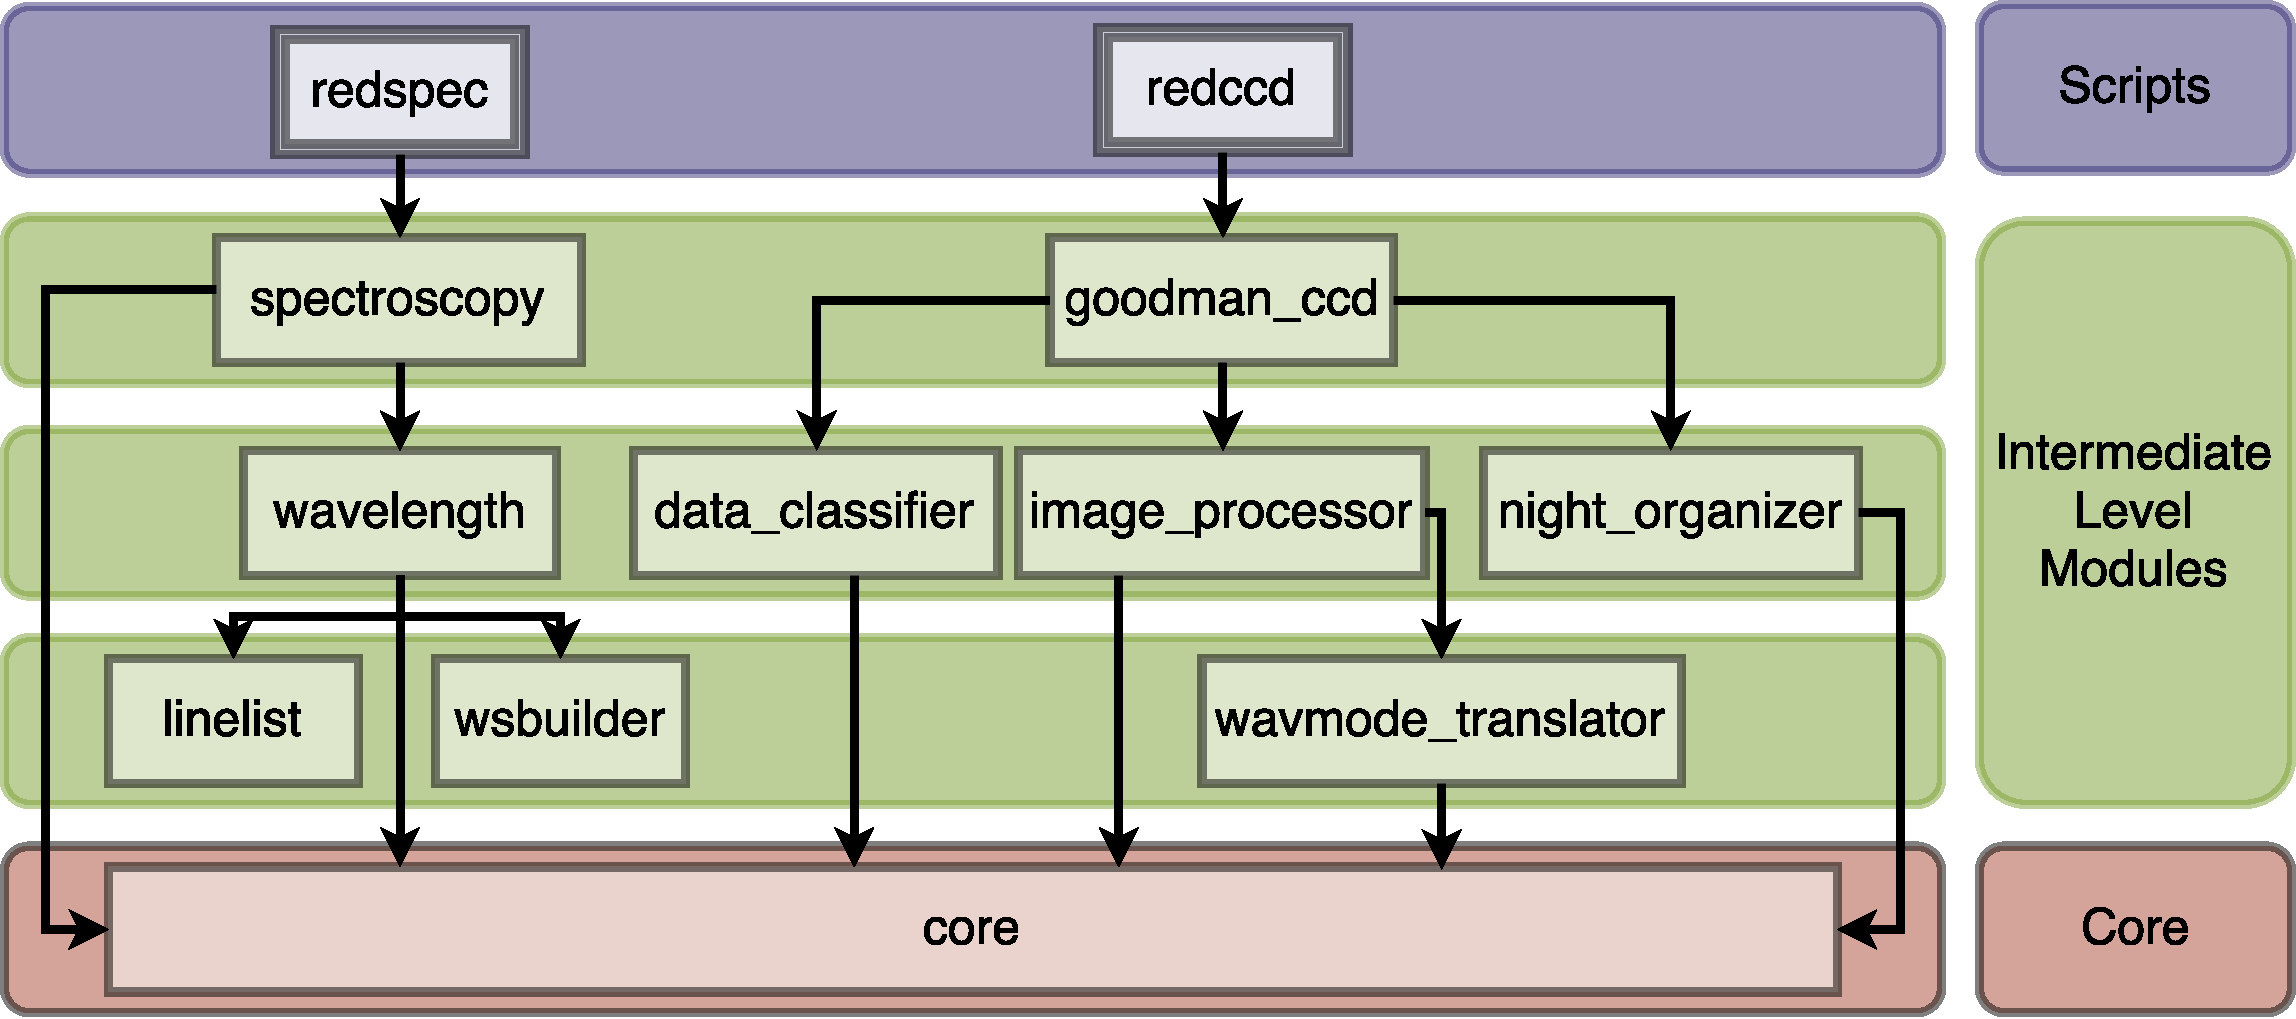
\includegraphics[width=0.95\linewidth]{P8989_f1.pdf}
\end{center}
}


\headerbox{5. Performance}{name=performance,span=2,column=1,below=concept}{ % To reduce this block to 1 column width, remove 'span=2'

\begin{center}
\begin{tabular}{|c|c|c|}
\hline
d& Automatic & Interactive\\
\hline
\hline
RMS Error & - & 4\\
\hline
Time & 1 & 1\\
\hline
\end{tabular}
\end{center}

% \begin{wrapfigure}{l}{0.3\textwidth}
%     \vspace{10pt}
%     \begin{center}
%         \includegraphics[width=\linewidth]{class}
%     \end{center}
%     %\vspace{-145pt}
% \end{wrapfigure}
% 
% % We tested DeCAF in 35 case studies taken from the DUD-E database, to evaluate its power to discriminate between active and inactive molecules.
% % We used DeCAF as a classifier and compared it to the SEA (Similarity Ensemble Approach) algorithm \cite{keiser2007relating}.
% % To compare sets of ligands, we adapted the approach used in SEA, replacing Tc by DCAF.
% % We prepared datasets as shown in the left diagram.
% % Then, we tested both classifiers calculating ROC AUC values for every target (below).
% We tested DeCAF in 35 diverse targets taken from the DUD-E database, to evaluate its power to classify molecules as active or inactive.
% We compared DeCAF to the renowned \textbf{SEA (Similarity Ensemble Approach)} algorithm \cite{keiser2007relating}, which uses Tc as a similarity measure.
% Dataset preparation steps are shown on the left diagram.
% Comparison results (\textbf{ROC AUC} values for each receptor) are shown below.
% % Please ask me about details.
% 
% \hspace{0pt}\includegraphics[width=0.95\linewidth]{res}

}


\headerbox{6. Results}{name=results,column=1,below=performance,span=2,above=bottom}{


\begin{center}
 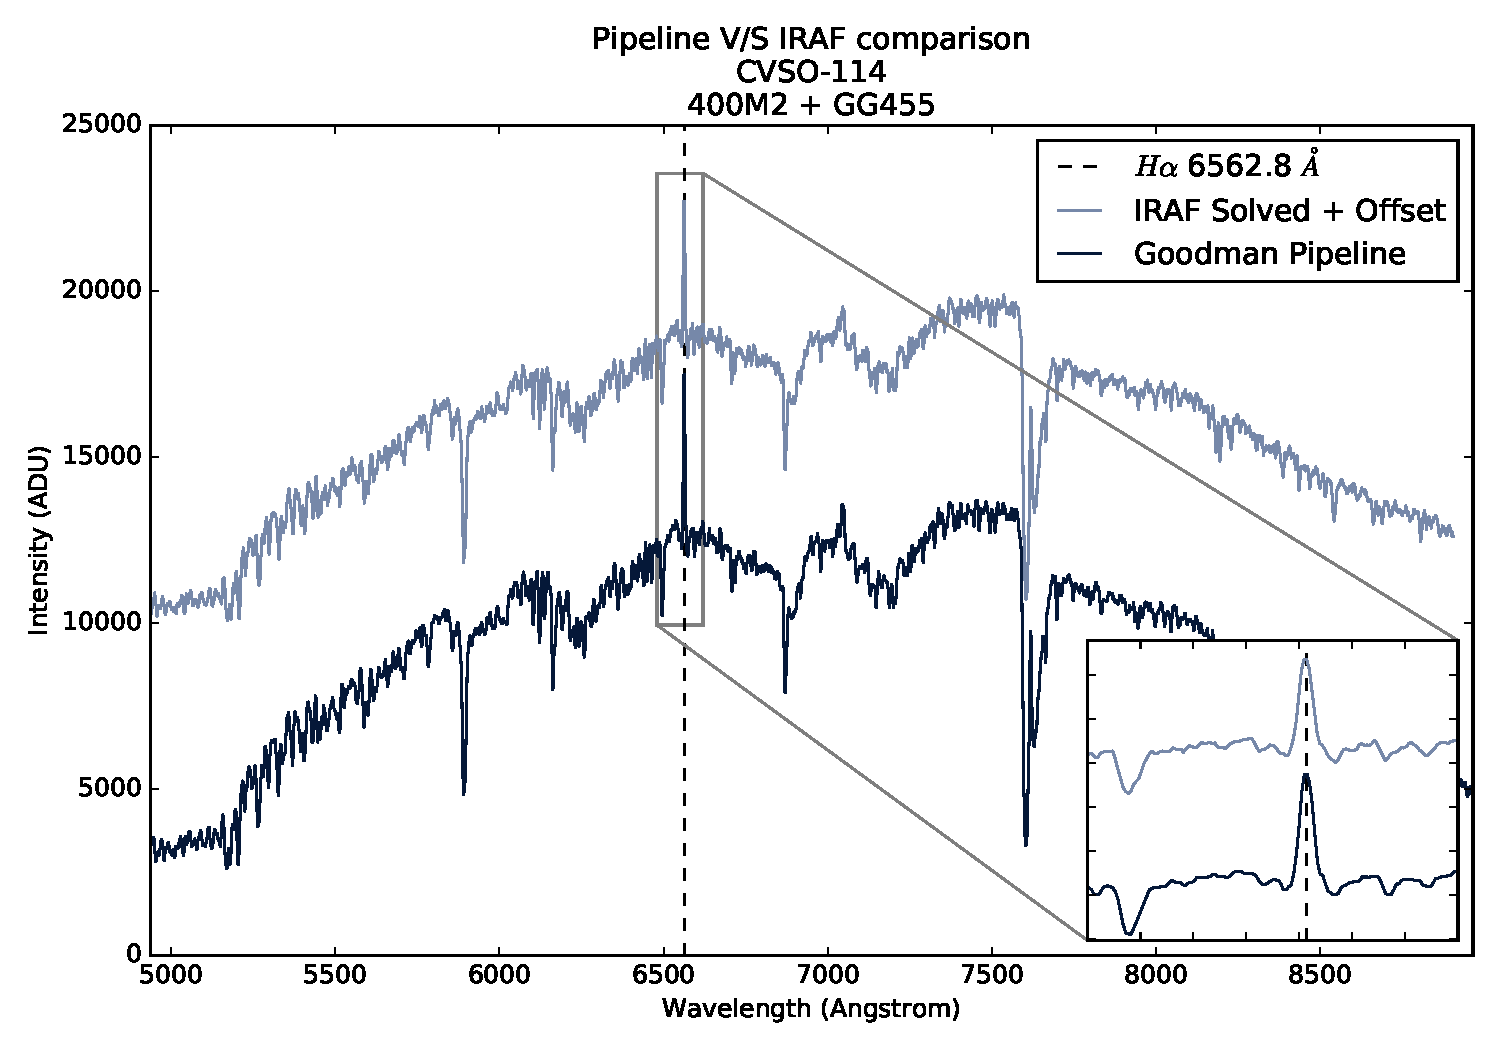
\includegraphics[width=0.95\linewidth]{P8989_f2.pdf}
\end{center}


}


\headerbox{7. References}{name=references,column=0,span=1,below=future,above=bottom}{


%\small % Reduce the font size in this block
\renewcommand{\section}[2]{\vskip 0.05em} % Get rid of the default "References" section title
%\nocite{*} % Insert publications even if they are not cited in the poster


\bibliographystyle{plain}
\bibliography{biblio} % Use sample.bib as the bibliography file
}

\end{poster}

\end{document}
